\chapter{Хоривица?}

Следуя предположению, что горой Хоривицей надо считать отрог, ныне слывущий частью Щекавицы, где расположены старообрядческое и мусульманское кладбища, отправимся туда. 

Добраться удобнее так – взойти на Щекавицу по улице Олеговской и шагать дальше, пока Олеговская не сольется с Лукьяновской, не станет ею. Справа будет сначала обрыв, превращенный в свалку – место бывшего татарского рынка Шурум-Бурум. Если не глядеть под ноги, открывается чудесный вид на зеленые остатки Лысой горы и Оболонь. В 2020 году глядеть уже нельзя – доступ к обрыву прегражден строительным забором. Но! Сейчас вроде бы 2013 год...

От обрыва до усадьбы мечети Ар-Рахма (переводится как «Милосердие», открыта в 2000 году) – труднопроходимые, замусоренные заросли. Далее на запад – сама мечеть, а точнее Исламский комплекс (доотвод земли около мечети – 2004 год, тогда же вероятно и начало строительства остальных зданий), включающий мечеть, медресе, минарет и Духовное Управление мусульман Украины.

Всё это соседствует западной же стороной с одной из террас отрога Хоривицы. Обозначим эту террасу буквой Б. По ней вдоль, на север, лежит мусульманское кладбище. За его восточным краем, склон резко сходит в глубокую низину Нижнеюрковского переулка. Далее кладбища мусульман, к северу, на той же высоте – плоский северный мыс Хоривицы, весьма примечательный, но туда мы заглянем позже.

На террасе выше Б – назовем эту новую террасу А, за бетонным забором – кладбище старообрядцев.

Туда ведут черные, двумя створками, кованные ворота на кладбище, а рядом такая же черная калитка. Нижняя половина – сплошная, верхняя – копья. Прежний вход на кладбище, разваленный в 1980-х, был ближе к перекрестку Лукьяновской и Олеговской улиц. До революции кладбище адресно относилось к Лукьяновскому переулку.

Заходим на кладбище. В тени деревьев, мимо старинных каменных надгробий движемся на север. Примерно так раньше выглядело и кладбище на Замковой горе, покуда там не порезвились вандалы. Только здесь – уклон в раскол. Купцы-староверы Булышкины, Поповы, Борисовы...

А вот западный склон Хоривицы лишен могил, и если глядеть на него снизу, с Нижнеюрковской – дик и зелен. Однако стоит посетить его, и вы увидите усеянную хламом гору, где на свободных пятачках древних укреплений суетятся хваткие шашлычники. Часть этой стороны горы, выходящая к улице Лукьяновской, подрезана линией гаражей. За нею еще западнее – здания ГАИ и его парковка, а позади них из Волчьего яра торчит в небо высоченная труба Лукьяновской котельной. Склон туда, за парковкой – свалка строительного мусора.

Терраса А имеет любопытное строение. Две широкие ее части соединены словно перешейком, как на горе Детинке. На дальнем, северном конце террасы А есть место, где старообрядческие, с характерными двуперстиями иконы, защищенные в эдаких маленьких домиках на столбиках, стоят украшенные цветами, рушниками и лампадками. Под столбиками растут цветы в ящиках. Обустроен нехитрый аналой, чтобы класть священные книги и вести богослужение.

\begin{center}
\includegraphics[width=\linewidth]{chast-kirvys/yourk/\myimgprefix 27082009599.jpg}
\end{center} 

%\begin{center}
%\includegraphics[width=\linewidth]{yourkovica/27082009592.jpg}
%\end{center} 

%\newpage

Возможно, эти столбики с иконами сооружены над безымянными захоронениями, поскольку неподалеку есть заросшая травой площадка со множеством могильных холмиков без каких-либо крестов и оград вообще.

Относительно братской, солдатской могилы в начале кладбища, по датам сужу, что многие бойцы Красной армии погибли от ранений после боев за Киев, в госпиталях. Вот имена героев, с общего надгробия (переписываю со сделанной мною фотографии):\\

\noindent
рядовой Алжбаев Г Р 1913-1944

\noindent
рядовой Арнеу Михаил Дмитриевич 1924-1944

\noindent
мл сержант Архипов Михаил Дмитриевич ?-1944

\noindent
рядовой Бельский Михаил Маркович 22.XI.1943

\noindent
рядовой Валько\footnote{Или Вальков.} Максим Семенович 1909- 22.XI.1943

\noindent
лейтенант Горочевский 1944

\noindent
лейтенант Гошаренко Юрий Иванович 1944

\noindent
рядовой Омеляненко Иван Исаевич 20.XI.1943

\noindent
ст сержант Халиков МА?? 20.XI.1943

\noindent
майор Цимбал Григорий Анисимович 16.XI.1943

\noindent
рядомой Яценко Михаил Иванович 1915-17.XI.1943

\noindent
рядовой Яценко Максим Иванович 1915-1944\\

Братские могилы бойцов Красной армии были найдены и приведены в порядок историко-культурным обществом «Старая Поляна» (названо по близлежащей местности) и историко-патриотическим клубом «Поиск». Деятельность эта ведется с 1990 года. Некоторые данные о погибших из архива Минобороны СССР:\\ 

\noindent
Архипов Михаил Дмитриевич, мл. сержант 70-й танковой бригады. Умер от ран 17.11.43 г. 

\noindent
Бельский Михаил Маркович, рядовой 340 стрелковой дивизии (по другим сведениям – сержант, см. Книга Памяти, Самарская область). Умер от ран 22.11.43 г. 

\noindent
Омеляненко Иван Исаевич, рядовой 1144 стрелкового полка. Погиб 20.11.43 г.

\noindent
Плаходный Платон Яковлевич, 1913 г.р., рядовой 1144 стрелкового полка. Погиб 22.11.43 г. 

\noindent
Халиков Мазиб, ст. сержант 1140 стрелкового полка, погиб 20.11.43 г.

\noindent
Яценко Максим Иванович, 1915 г.р., из села Клеховка Фастовского района Киевской области, рядовой 232 стрелковой дивизии. Умер от ран 17.11.43 г. 

\noindent
Яценко Михаил Иванович, 1915 г.р., рядовой 791 стрелкового полка 135 стрелковой дивизии. Погиб в 1944 г.\\

%Есть на кладбище и одна младенческая могилка военных лет, Аллы Владимировны Трофимоновой, которая родилась в 1944 году, и в августе умерла. 

Но это у входа. А пройди чуть дальше. Старые, тяжелые памятники из черного камня соседствуют тут с участками, где среди сорной травы торчат обычные «латинские», без перекладин, кресты – некоторым из них придан «старообрядческий» вид при помощи проволоки или венков. Одни кресты выкрашены серебрянкой и обсажены ландышами, другие просто ржавеют в отдалении. Могилу юродивого Ивана Босого посещают, вероятно, чаще всего. На ней лежат подношения – яблоки и прочая снедь.

Когда же появилось старообрядческое кладбище? На толковейшей карте 1803 года, составленной Андреем Меленским, гора еще дикая. А вот на плане окрестностей Киева, за 1842-й, по современному нам месту старообрядческого кладбища, однако не углубляясь на сам отрог, уже крестиками обозначено кладбище, без подписи.

На карте 1860 года тоже есть отделенное от основного, но не меньшее, старообрядческое, да названы Щекавица и Юрковица (сложно понять к чему точно относится последняя надпись, склоны туда и сюда от удолья с котельной Лукьяновской, скажем так, включая «старообрядческий» отрог).

\begin{center}
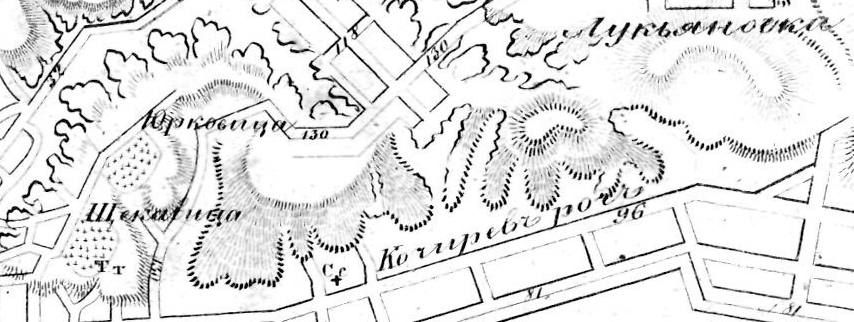
\includegraphics[width=\linewidth]{chast-kirvys/yourk/1860-part.jpg}
\end{center} 

Местность, слывущая ныне как низовье Кирилловских высот, тут подписана «Копиревъ рогъ», что явно имеет отношение к Копыреву концу. Лукьяновкой же подписана местность, известная ныне как Татарка (современная Татарка граничит с Лукьяновкой, отделяясь от нее глубоким Кмитовым яром, в котором расположен завод Артёма). И по представлениям киевлян 19 века, это всё была Лукьяновка.

%Там, именно там, Хвойка нашел свою Кирилловскую стоянку, там в пещерке отыскали обескровленное, измученное тело Андрюши Ющинского, известное по делу Бейлиса, там, далее – Логово Змиево.

На карте 1865 года, в тех же пределах что и в 1860, изображено «Староверческое кладбище», а отрог холма за ним подписан «Юрковица».
  
С горы далеко видны окрестности – вся Оболонь, соседняя Лысая гора (современная Юрковица), обращенная к Хоривице стороной, где расположена воинская часть и заброшенный кирпичный завод.

Подножие Хоривицы – прежние Рогатки – огибается, с востока, Нижнеюрковским переулком, а с севера и запада Нижнеюрковской улицей. Переулок издавна, по крайней мере в 19 веке, был населен, стояли частные домики. Теперь он занят лентоткацкой фабрикой, недостроенным зданием и баром, музыка с которого разносится по всей округе. 

Под юго-западной стороной горы высится трубой в небо котельная «Лукьяновская».

Снимок 2009 года, сделанный с Террасы А Хоривицы: 

\begin{center}
\includegraphics[width=\linewidth]{chast-kirvys/yourk/\myimgprefix 27082009589.jpg}
\end{center} 

Перед нами, в кадре по правую руку внизу, и там где мы стоим – Хоривица, а слева за трубой и справа за сооружениями – гора Лысая-Юрковица. Полосатая труба это не от Лукьяновской котельной. 

Справа же, светлое здание рядом с домом, у которого красненькая крыша – элеватор Пивзавода на Подоле. Элеватор стоит на четной стороне улицы Кирилловской, а пивзавод – на нечетной. В 2014 году здания пивзавода были выставлены на продажу.

\begin{center}
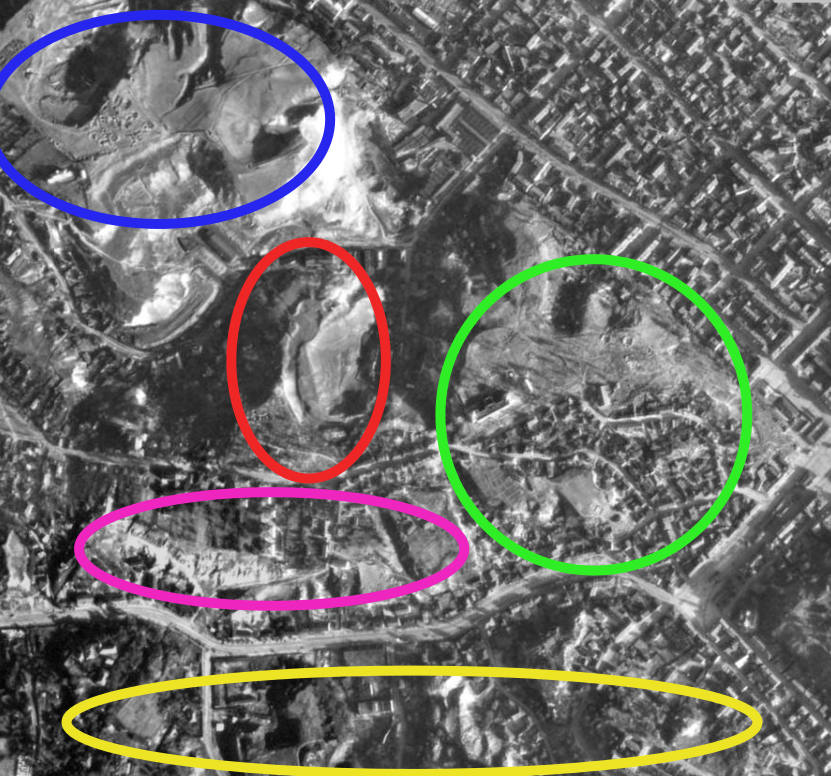
\includegraphics[width=\linewidth]{chast-kirvys/yourk/y.jpg}
\end{center} 

На аэрофотоснимке 1943 года я отметил овалами следующее. Желтый – склоны Кудрявца в общепринятой трактовке. Зеленый – Щекавица. Малиновый – я не знаю, как это назвать, но скорее всего тоже Щекавица\footnote{Обратите внимание на ровные яры в правом конце малинового овала – это же древние рвы! Сейчас это окрестности Лукьяновского переулка.}). Между зеленым, малиновым и желтым – улица Глубочицкая. Красный – Хоривица. Синий – Лысая-Юрковица.

О Хоривице я могу рассказать очень мало. Привычная трактовка её краеведами как части Щекавицы, примечательной кладбищем старообрядцев, не воодушевляла исследователей. А устроение там кладбищ и зданий уничтожило древние культурные слои на большой части горы.

Кроме пещер наверху Щекавицы и Хоривицы, какие-то пещеры были и на склоне внизу у самой Рогатки, на углу Нижнеюрковского переулка и Нижнеюрковской улицы, примерно по современному №9.

Терраса Б выдается на север много дальше Террасы А. Самый северный мыс горы, на уровне Террасы Б ограничен валами, под восточным из которых тоже есть терраса, обозначим ее буквой В. Поверхность мыса, в отличие от его склонов, лишена деревьев и поросла густой травой. Всюду следы чего-то древнего – ровные углубления, возвышения, переходы.

Удивляет земляной бассейн – прямоугольное большое углубление на плато. Дно заболочено полувысохшим родником, питаемым вероятно за счет водного горизонта Террасы А, ведь Терраса Б лежит ниже. Это могло быть хранилище воды для древней крепости, наполняемое родником и дождями. Либо бассейн под открытым небом служил предметом особой роскоши, восьмым чудом света. 

\begin{center}
\includegraphics[width=\linewidth]{chast-kirvys/yourk/\myimgprefix IMG_20160605_144808.jpg}

\textit{Вид на бассейн с северо-запада. Слева – труба Лукьяновской котельной.}
\end{center}

\begin{center}
\includegraphics[width=\linewidth]{chast-kirvys/yourk/\myimgprefix IMG_20160605_145830.jpg}

\textit{Снова бассейн. Вид на юг, в сторону мечети.}
\end{center}

\begin{center}
\includegraphics[width=\linewidth]{chast-kirvys/yourk/\myimgprefix IMG_20160605_145810.jpg}

\textit{Стою в бассейне. Вид на восток.}
\end{center}

\newpage

\begin{center}
\includegraphics[width=0.90\linewidth]{chast-kirvys/yourk/\myimgprefix IMG_20160605_144812.jpg}

\textit{Вид с восточного склона на противоположный, Щекавицу. Слева – участок, где пещера за школой. Внизу – переулок Нижнеюрковский.}
\end{center}

\begin{center}
\includegraphics[width=0.90\linewidth]{chast-kirvys/yourk/\myimgprefix IMG_20160605_144814.jpg}

\textit{Вид туда же, объектив смещен правее. Видна вся котловина между отрогами. Большая залысина в левой части кадра – обрыв со свалкой у Шурум-Бурума.}
\end{center}

\newpage

\begin{center}
\includegraphics[width=0.98\linewidth]{chast-kirvys/yourk/\myimgprefix IMG_20160605_144819.jpg}

\textit{Вид на северо-восток. Выемка – не бассейн.}
\end{center}

\begin{center}
\includegraphics[width=0.98\linewidth]{chast-kirvys/yourk/\myimgprefix IMG_20160605_144820.jpg}

\textit{По восточному склону вперед, на северо-восток, идет вал.}
\end{center}

\newpage

\begin{center}
\includegraphics[width=0.94\linewidth]{chast-kirvys/yourk/\myimgprefix IMG_20160605_145141.jpg}

\textit{Вид на конец этого вала с нижележащей Террасы В.}
\end{center}


\begin{center}
\includegraphics[width=0.94\linewidth]{chast-kirvys/yourk/\myimgprefix IMG_20160605_145220.jpg}

\textit{Вид с Террасы В в другую сторону, на ул. Нижнеюрковскую. Гостинка справа – №13. Слева – общага (здание №4), потом трубы кирпичного и пивного заводов.}
\end{center}

\newpage

\begin{center}
\includegraphics[width=0.90\linewidth]{chast-kirvys/yourk/\myimgprefix IMG_20160605_145437.jpg}

\textit{Вид с северного мыса левее, на север. Прямо – место срытой кирпичным заводом части холма Лысой-Юрковицы.}
\end{center}


\begin{center}
\includegraphics[width=0.90\linewidth]{chast-kirvys/yourk/\myimgprefix IMG_20160605_150002.jpg}

\textit{Вид вдоль западного склона Хоривицы на юго-запад. Справа внизу – яр, оттуда торчит труба Лукьяновской котельной.}
\end{center}

\newpage

\begin{center}
\includegraphics[width=\linewidth]{chast-kirvys/yourk/\myimgprefix IMG_20160605_150112.jpg}

\textit{Вид вдоль западного склона Хоривицы на северо-восток.}
\end{center}

%\begin{center}
%\includegraphics[width=\linewidth]{yourkovica/\myimgprefix IMG_20160605_144319.jpg}

%Вид на Террасу А с Террасы Б.
%\end{center}

%Не стоит обольщаться, что исконная Юрковица сохранится надолго, покуда ее ограничивают кладбища со стороны Лукьяновской улицы. 

%Уже сейчас по некоторым участкам склона стоят красные металлические двуноги с прикрученными шурупами досками, надписи на коих гласят: «Обережно зсув грунта», причем буква «з» почему-то повернута в сторону, противную обычной. Склепать эти двуноги, затащить наверх и поставить сил хватило, а укрепить склоны под указанными местами – нет.

%Если снизу на Нижнеюрковской или в Нижнеюрковском переулке затеют какое-нибудь строительство – а малоэтажная застройка, сохраняемая по начало 21 века, к тому коммерчески располагает – то этих оползней грунта будет столько, что двуног не хватит.

Местность сию, запечатленную на видео, можно посмотреть в серии «Киевской амплитуды» под названием «Забытые подземелья Киева».

%Осенью 2016 года весь северный отрог – с бассейном и валами – оказался отгороженным от старообрядческого кладбища зеленым металлическим забором.

Перелетим к соседней, лежащей отсюда на север, Лысой горе.